%TEX root = ./overwiew.tex

\documentclass{standalone}
% http://texample.net/tikz/examples/inertial-navigation-system/

\usepackage{tikz}
\usetikzlibrary{positioning}
\usetikzlibrary{shapes,arrows}
\usetikzlibrary{arrows.meta, positioning, quotes}

\begin{document}

\tikzstyle{module}=[draw, fill=blue!20, text width=5em, text centered, minimum height=2cm]
\tikzstyle{module_def}=[fill=yellow!20,rounded corners, draw=black!50, dashed]
\tikzstyle{signal_name} = [above, text width=10em]
\tikzstyle{module_name} = [above right, text width=10em]
\tikzstyle{spn_node} = [draw, circle, fill=green!20, minimum width=0.5cm]
\tikzstyle{sy} = [yshift=#1mm]

% \def\blockdist{3.5cm}
% \def\edgedist{1.5cm}

\pgfdeclarelayer{background}
\pgfdeclarelayer{foreground}
\pgfsetlayers{background,main,foreground}

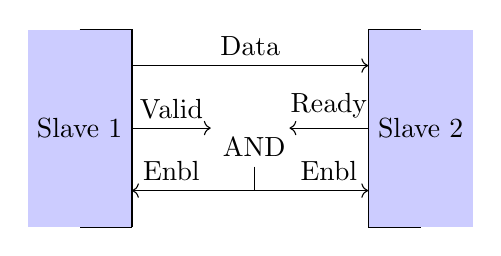
\begin{tikzpicture}

	\node (slave_1) [fill=blue!20, minimum height=2.5cm] {Slave 1};
	\node (slave_2) [fill=blue!20, minimum height=2.5cm, right=3cm of slave_1] {Slave 2};

	\path[draw] (slave_1.north) -- (slave_1.east |- slave_1.north);
	\path[draw] (slave_1.east |- slave_1.north) -- (slave_1.east |- slave_1.south);
	\path[draw] (slave_1.east |- slave_1.south) -- (slave_1.south);

	\path[draw] (slave_2.north) -- (slave_2.west |- slave_2.north);
	\path[draw] (slave_2.west |- slave_2.north) -- (slave_2.west |- slave_2.south);
	\path[draw] (slave_2.west |- slave_2.south) -- (slave_2.south);

	\path[draw, ->] (slave_1.50) -- node[above] {Data} (slave_2.130);
	\node (n11) [right=1cm of slave_1] {};
	\path[draw, ->] (slave_1.0) -- node[above] {Valid} (n11);
	\node (n12) [right=1cm of slave_1.-50] {};
	\path[draw, ->] (n12) -- node[above] {Enbl} (slave_1.-50);

	\node (n21) [left=1cm of slave_2] {};
	\node (n22) [left=1cm of slave_2.-130] {};
	\path [draw, ->] (slave_2) -- node[above] {Ready} (n21);
	\path [draw, ->] (n22) -- node[above] {Enbl} (slave_2.-130);
	\node (and) [left=0.2cm of n21, below] {AND};
	\path [draw] (and) -- (n12 -| and);
	\path [draw] (n12.west) -- (n22.east);
	% \node (root) [spn_node] {$+$};

	% \node (x2) [spn_node, below=0.7cm of root] {$\times$};
	% \node (x1) [spn_node, left=2cm of x2] {$\times$};
	% \node (x3) [spn_node, right=2cm of x2] {$\times$};

	% \node (p1) [spn_node, below=0.5cm of x1] {$+$};
	% \node (p2) [spn_node, right=1cm of p1] {$+$};
	% \node (p4) [spn_node, below=0.5cm of x3] {$+$};
	% \node (p3) [spn_node, left=1cm of p4] {$+$};

	% \node (l1) [below=1cm of p1] {$X_1$};
	% \node (l2) [below=1cm of p2] {$\bar{X_1}$};
	% \node (l3) [below=1cm of p3] {$X_2$};
	% \node (l4) [below=1cm of p4] {$\bar{X_2}$};

	% \path[draw] (x1) -- node[above] {0.5} (root);
	% \path[draw] (x2) -- node[left] {0.2} (root);
	% \path[draw] (x3) -- node[above] {0.3} (root);

	% \path [draw] (p1) -- (x1);
	% \path [draw] (p1) -- (x2);
	% \path [draw] (p2) -- (x3);
	% \path [draw] (p3) -- (x1);
	% \path [draw] (p4) -- (x2);
	% \path [draw] (p4) -- (x3);

	% \path [draw] (l1) -- node[left] {0.6} (p1);
	% \path [draw] (l1) -- node[left] {} (p2);
	% \path [draw] (l2) -- node[right] {} (p1);
	% \path [draw] (l2) -- node[right] {0.1} (p2);

	% \path [draw] (l3) -- node[left] {0.3} (p3);
	% \path [draw] (l3) -- node[left] {} (p4);
	% \path [draw] (l4) -- node[right] {} (p3);
	% \path [draw] (l4) -- node[right] {0.8} (p4);

	% \node (input) [module, minimum width=2cm, minimum height=8cm] {};
	% \node () [rotate=90] at (input) {Input module};

	% \node (spn)[module, minimum width=6cm, minimum height=6cm, above right=-6cm and 1cm of input] {};
	% \node [below right=-0.7cm and -1cm of spn] {SPN};


	% \node (ctrl)[module,minimum width=2cm,minimum height=2.2cm,above right=-2.2cm and 2cm of spn] {Control};
	% \node (mem)[module, minimum width=2cm,minimum height=4cm,below=1.5cm of ctrl] {RAM};


\end{tikzpicture}

\end{document}

